\documentclass{standalone}
\usepackage{tikz}
\usetikzlibrary{patterns, positioning}

\begin{document}
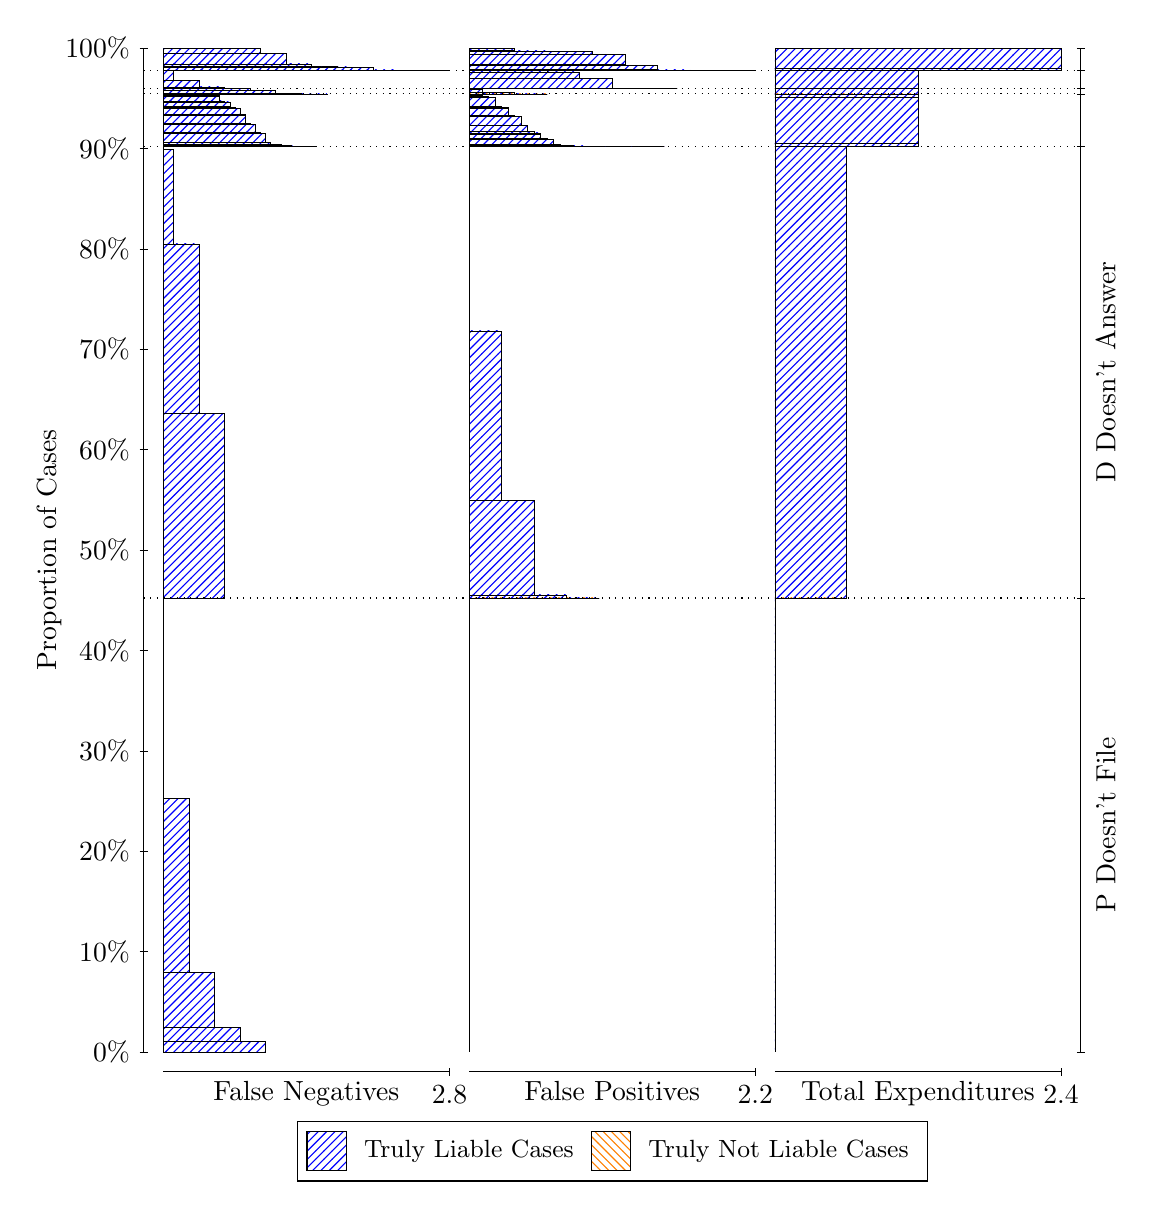
\begin{tikzpicture}
\draw[black, very thin] (1.5,1.75) -- (1.5,14.5);
\node[rotate=90, anchor=center] at (0.3, 8.125) {Proportion of Cases};
\draw[black, very thin] (1.45,1.75) -- (1.55,1.75);
\node[anchor=east] at (1.45, 1.75) {0\%};
\draw[black, very thin] (1.45,3.025) -- (1.55,3.025);
\node[anchor=east] at (1.45, 3.025) {10\%};
\draw[black, very thin] (1.45,4.3) -- (1.55,4.3);
\node[anchor=east] at (1.45, 4.3) {20\%};
\draw[black, very thin] (1.45,5.575) -- (1.55,5.575);
\node[anchor=east] at (1.45, 5.575) {30\%};
\draw[black, very thin] (1.45,6.85) -- (1.55,6.85);
\node[anchor=east] at (1.45, 6.85) {40\%};
\draw[black, very thin] (1.45,8.125) -- (1.55,8.125);
\node[anchor=east] at (1.45, 8.125) {50\%};
\draw[black, very thin] (1.45,9.4) -- (1.55,9.4);
\node[anchor=east] at (1.45, 9.4) {60\%};
\draw[black, very thin] (1.45,10.675) -- (1.55,10.675);
\node[anchor=east] at (1.45, 10.675) {70\%};
\draw[black, very thin] (1.45,11.95) -- (1.55,11.95);
\node[anchor=east] at (1.45, 11.95) {80\%};
\draw[black, very thin] (1.45,13.225) -- (1.55,13.225);
\node[anchor=east] at (1.45, 13.225) {90\%};
\draw[black, very thin] (1.45,14.5) -- (1.55,14.5);
\node[anchor=east] at (1.45, 14.5) {100\%};

\draw[black, very thin] (13.4,1.75) -- (13.4,14.5);
\draw[black, very thin] (13.35,1.75) -- (13.45,1.75);
\node[anchor=west] at (13.35, 1.75) {};
\draw[black, very thin] (13.35,7.5159) -- (13.45,7.5159);
\node[anchor=west] at (13.35, 7.5159) {};
\draw[black, very thin] (13.35,13.254) -- (13.45,13.254);
\node[anchor=west] at (13.35, 13.254) {};
\draw[black, very thin] (13.35,13.917) -- (13.45,13.917);
\node[anchor=west] at (13.35, 13.917) {};
\draw[black, very thin] (13.35,13.987) -- (13.45,13.987);
\node[anchor=west] at (13.35, 13.987) {};
\draw[black, very thin] (13.35,14.217) -- (13.45,14.217);
\node[anchor=west] at (13.35, 14.217) {};
\draw[black, very thin] (13.35,14.5) -- (13.45,14.5);
\node[anchor=west] at (13.35, 14.5) {};

\draw[black, very thin, pattern color=blue, pattern=north east lines] (1.75,1.75) rectangle (3.0476,1.8807);
\draw[black, very thin, pattern color=blue, pattern=north east lines] (1.75,1.8807) rectangle (2.7232,2.0577);
\draw[black, very thin, pattern color=blue, pattern=north east lines] (1.75,2.0577) rectangle (2.3988,2.7603);
\draw[black, very thin, pattern color=blue, pattern=north east lines] (1.75,2.7603) rectangle (2.0744,4.9694);
\draw[black, very thin, pattern color=orange, pattern=north west lines] (1.75,4.9694) rectangle (1.75,4.9694);
\draw[black, very thin, pattern color=blue, pattern=north east lines] (1.75,4.9694) rectangle (1.75,7.5159);
\draw[black, very thin, pattern color=blue, pattern=north east lines] (1.75,7.5159) rectangle (2.5286,9.8621);
\draw[black, very thin, pattern color=blue, pattern=north east lines] (1.75,9.8621) rectangle (2.2042,12.014);
\draw[black, very thin, pattern color=blue, pattern=north east lines] (1.75,12.014) rectangle (1.8798,13.214);
\draw[black, very thin, pattern color=orange, pattern=north west lines] (1.75,13.214) rectangle (1.75,13.214);
\draw[black, very thin, pattern color=blue, pattern=north east lines] (1.75,13.214) rectangle (1.75,13.254);
\draw[black, very thin, pattern color=blue, pattern=north east lines] (1.75,13.254) rectangle (3.6964,13.254);
\draw[black, very thin, pattern color=blue, pattern=north east lines] (1.75,13.254) rectangle (3.5667,13.255);
\draw[black, very thin, pattern color=blue, pattern=north east lines] (1.75,13.255) rectangle (3.4369,13.256);
\draw[black, very thin, pattern color=blue, pattern=north east lines] (1.75,13.256) rectangle (3.372,13.266);
\draw[black, very thin, pattern color=blue, pattern=north east lines] (1.75,13.266) rectangle (3.3071,13.267);
\draw[black, very thin, pattern color=blue, pattern=north east lines] (1.75,13.267) rectangle (3.2423,13.276);
\draw[black, very thin, pattern color=blue, pattern=north east lines] (1.75,13.276) rectangle (3.1774,13.281);
\draw[black, very thin, pattern color=blue, pattern=north east lines] (1.75,13.281) rectangle (3.1125,13.299);
\draw[black, very thin, pattern color=blue, pattern=north east lines] (1.75,13.299) rectangle (3.0476,13.417);
\draw[black, very thin, pattern color=blue, pattern=north east lines] (1.75,13.417) rectangle (2.9827,13.427);
\draw[black, very thin, pattern color=blue, pattern=north east lines] (1.75,13.427) rectangle (2.9179,13.434);
\draw[black, very thin, pattern color=blue, pattern=north east lines] (1.75,13.434) rectangle (2.9179,13.528);
\draw[black, very thin, pattern color=blue, pattern=north east lines] (1.75,13.528) rectangle (2.853,13.541);
\draw[black, very thin, pattern color=blue, pattern=north east lines] (1.75,13.541) rectangle (2.7881,13.651);
\draw[black, very thin, pattern color=blue, pattern=north east lines] (1.75,13.651) rectangle (2.7881,13.656);
\draw[black, very thin, pattern color=blue, pattern=north east lines] (1.75,13.656) rectangle (2.7232,13.731);
\draw[black, very thin, pattern color=blue, pattern=north east lines] (1.75,13.731) rectangle (2.6583,13.748);
\draw[black, very thin, pattern color=blue, pattern=north east lines] (1.75,13.748) rectangle (2.5935,13.76);
\draw[black, very thin, pattern color=blue, pattern=north east lines] (1.75,13.76) rectangle (2.5935,13.816);
\draw[black, very thin, pattern color=blue, pattern=north east lines] (1.75,13.816) rectangle (2.5286,13.829);
\draw[black, very thin, pattern color=blue, pattern=north east lines] (1.75,13.829) rectangle (2.4637,13.887);
\draw[black, very thin, pattern color=blue, pattern=north east lines] (1.75,13.887) rectangle (2.4637,13.896);
\draw[black, very thin, pattern color=blue, pattern=north east lines] (1.75,13.896) rectangle (2.3988,13.904);
\draw[black, very thin, pattern color=blue, pattern=north east lines] (1.75,13.904) rectangle (2.3339,13.904);
\draw[black, very thin, pattern color=blue, pattern=north east lines] (1.75,13.904) rectangle (2.3339,13.909);
\draw[black, very thin, pattern color=blue, pattern=north east lines] (1.75,13.909) rectangle (2.269,13.912);
\draw[black, very thin, pattern color=blue, pattern=north east lines] (1.75,13.912) rectangle (2.269,13.912);
\draw[black, very thin, pattern color=blue, pattern=north east lines] (1.75,13.912) rectangle (2.2042,13.913);
\draw[black, very thin, pattern color=blue, pattern=north east lines] (1.75,13.913) rectangle (2.1393,13.914);
\draw[black, very thin, pattern color=blue, pattern=north east lines] (1.75,13.914) rectangle (2.1393,13.915);
\draw[black, very thin, pattern color=blue, pattern=north east lines] (1.75,13.915) rectangle (2.0744,13.916);
\draw[black, very thin, pattern color=blue, pattern=north east lines] (1.75,13.916) rectangle (2.0095,13.916);
\draw[black, very thin, pattern color=blue, pattern=north east lines] (1.75,13.916) rectangle (2.0095,13.917);
\draw[black, very thin, pattern color=blue, pattern=north east lines] (1.75,13.917) rectangle (1.9446,13.917);
\draw[black, very thin, pattern color=blue, pattern=north east lines] (1.75,13.917) rectangle (1.8798,13.917);
\draw[black, very thin, pattern color=blue, pattern=north east lines] (1.75,13.917) rectangle (1.8149,13.917);
\draw[black, very thin, pattern color=orange, pattern=north west lines] (1.75,13.917) rectangle (1.75,13.917);
\draw[black, very thin, pattern color=blue, pattern=north east lines] (1.75,13.917) rectangle (1.75,13.917);
\draw[black, very thin, pattern color=blue, pattern=north east lines] (1.75,13.917) rectangle (3.8262,13.918);
\draw[black, very thin, pattern color=blue, pattern=north east lines] (1.75,13.918) rectangle (3.5018,13.925);
\draw[black, very thin, pattern color=blue, pattern=north east lines] (1.75,13.925) rectangle (3.1774,13.962);
\draw[black, very thin, pattern color=blue, pattern=north east lines] (1.75,13.962) rectangle (2.853,13.986);
\draw[black, very thin, pattern color=blue, pattern=north east lines] (1.75,13.986) rectangle (2.5286,13.987);
\draw[black, very thin, pattern color=orange, pattern=north west lines] (1.75,13.987) rectangle (1.75,13.987);
\draw[black, very thin, pattern color=blue, pattern=north east lines] (1.75,13.987) rectangle (2.5286,14.006);
\draw[black, very thin, pattern color=blue, pattern=north east lines] (1.75,14.006) rectangle (2.2042,14.088);
\draw[black, very thin, pattern color=blue, pattern=north east lines] (1.75,14.088) rectangle (1.8798,14.213);
\draw[black, very thin, pattern color=orange, pattern=north west lines] (1.75,14.213) rectangle (1.75,14.213);
\draw[black, very thin, pattern color=blue, pattern=north east lines] (1.75,14.213) rectangle (1.75,14.217);
\draw[black, very thin, pattern color=blue, pattern=north east lines] (1.75,14.217) rectangle (5.3833,14.217);
\draw[black, very thin, pattern color=blue, pattern=north east lines] (1.75,14.217) rectangle (5.0589,14.217);
\draw[black, very thin, pattern color=blue, pattern=north east lines] (1.75,14.217) rectangle (4.7345,14.221);
\draw[black, very thin, pattern color=blue, pattern=north east lines] (1.75,14.221) rectangle (4.4101,14.252);
\draw[black, very thin, pattern color=blue, pattern=north east lines] (1.75,14.252) rectangle (4.2804,14.252);
\draw[black, very thin, pattern color=blue, pattern=north east lines] (1.75,14.252) rectangle (4.0857,14.261);
\draw[black, very thin, pattern color=blue, pattern=north east lines] (1.75,14.261) rectangle (3.956,14.262);
\draw[black, very thin, pattern color=blue, pattern=north east lines] (1.75,14.262) rectangle (3.7613,14.262);
\draw[black, very thin, pattern color=blue, pattern=north east lines] (1.75,14.262) rectangle (3.6315,14.298);
\draw[black, very thin, pattern color=blue, pattern=north east lines] (1.75,14.298) rectangle (3.4369,14.298);
\draw[black, very thin, pattern color=blue, pattern=north east lines] (1.75,14.298) rectangle (3.3071,14.435);
\draw[black, very thin, pattern color=blue, pattern=north east lines] (1.75,14.435) rectangle (2.9827,14.495);
\draw[black, very thin, pattern color=blue, pattern=north east lines] (1.75,14.495) rectangle (2.6583,14.5);
\draw[black, very thin, pattern color=blue, pattern=north east lines] (1.75,14.5) rectangle (2.3339,14.5);
\draw[black, very thin, pattern color=blue, pattern=north east lines] (1.75,14.5) rectangle (2.0095,14.5);
\draw[black, very thin, pattern color=orange, pattern=north west lines] (1.75,14.5) rectangle (1.75,14.5);
\draw[black, very thin, pattern color=orange, pattern=north west lines] (5.6333,1.75) rectangle (5.6333,1.75);
\draw[black, very thin, pattern color=blue, pattern=north east lines] (5.6333,1.75) rectangle (5.6333,7.5159);
\draw[black, very thin, pattern color=orange, pattern=north west lines] (5.6333,7.5159) rectangle (7.2848,7.5159);
\draw[black, very thin, pattern color=blue, pattern=north east lines] (5.6333,7.5159) rectangle (7.2848,7.5159);
\draw[black, very thin, pattern color=blue, pattern=north east lines] (5.6333,7.5159) rectangle (6.872,7.5558);
\draw[black, very thin, pattern color=blue, pattern=north east lines] (5.6333,7.5558) rectangle (6.4591,8.7554);
\draw[black, very thin, pattern color=blue, pattern=north east lines] (5.6333,8.7554) rectangle (6.0462,10.908);
\draw[black, very thin, pattern color=blue, pattern=north east lines] (5.6333,10.908) rectangle (5.6333,13.254);
\draw[black, very thin, pattern color=orange, pattern=north west lines] (5.6333,13.254) rectangle (8.1106,13.254);
\draw[black, very thin, pattern color=blue, pattern=north east lines] (5.6333,13.254) rectangle (8.1106,13.254);
\draw[black, very thin, pattern color=orange, pattern=north west lines] (5.6333,13.254) rectangle (7.9455,13.254);
\draw[black, very thin, pattern color=blue, pattern=north east lines] (5.6333,13.254) rectangle (7.9455,13.254);
\draw[black, very thin, pattern color=orange, pattern=north west lines] (5.6333,13.254) rectangle (7.7803,13.254);
\draw[black, very thin, pattern color=blue, pattern=north east lines] (5.6333,13.254) rectangle (7.7803,13.254);
\draw[black, very thin, pattern color=blue, pattern=north east lines] (5.6333,13.254) rectangle (7.6977,13.254);
\draw[black, very thin, pattern color=orange, pattern=north west lines] (5.6333,13.254) rectangle (7.6152,13.254);
\draw[black, very thin, pattern color=blue, pattern=north east lines] (5.6333,13.254) rectangle (7.6152,13.254);
\draw[black, very thin, pattern color=blue, pattern=north east lines] (5.6333,13.254) rectangle (7.5326,13.254);
\draw[black, very thin, pattern color=orange, pattern=north west lines] (5.6333,13.254) rectangle (7.45,13.254);
\draw[black, very thin, pattern color=blue, pattern=north east lines] (5.6333,13.254) rectangle (7.45,13.254);
\draw[black, very thin, pattern color=blue, pattern=north east lines] (5.6333,13.254) rectangle (7.3674,13.254);
\draw[black, very thin, pattern color=orange, pattern=north west lines] (5.6333,13.254) rectangle (7.2848,13.254);
\draw[black, very thin, pattern color=blue, pattern=north east lines] (5.6333,13.254) rectangle (7.2848,13.255);
\draw[black, very thin, pattern color=blue, pattern=north east lines] (5.6333,13.255) rectangle (7.2023,13.255);
\draw[black, very thin, pattern color=orange, pattern=north west lines] (5.6333,13.255) rectangle (7.1197,13.255);
\draw[black, very thin, pattern color=blue, pattern=north east lines] (5.6333,13.255) rectangle (7.1197,13.258);
\draw[black, very thin, pattern color=blue, pattern=north east lines] (5.6333,13.258) rectangle (7.0371,13.258);
\draw[black, very thin, pattern color=orange, pattern=north west lines] (5.6333,13.258) rectangle (6.9545,13.258);
\draw[black, very thin, pattern color=blue, pattern=north east lines] (5.6333,13.258) rectangle (6.9545,13.259);
\draw[black, very thin, pattern color=blue, pattern=north east lines] (5.6333,13.259) rectangle (6.9545,13.262);
\draw[black, very thin, pattern color=blue, pattern=north east lines] (5.6333,13.262) rectangle (6.872,13.267);
\draw[black, very thin, pattern color=orange, pattern=north west lines] (5.6333,13.267) rectangle (6.7894,13.267);
\draw[black, very thin, pattern color=blue, pattern=north east lines] (5.6333,13.267) rectangle (6.7894,13.275);
\draw[black, very thin, pattern color=blue, pattern=north east lines] (5.6333,13.275) rectangle (6.7068,13.342);
\draw[black, very thin, pattern color=blue, pattern=north east lines] (5.6333,13.342) rectangle (6.6242,13.355);
\draw[black, very thin, pattern color=blue, pattern=north east lines] (5.6333,13.355) rectangle (6.5417,13.411);
\draw[black, very thin, pattern color=blue, pattern=north east lines] (5.6333,13.411) rectangle (6.5417,13.423);
\draw[black, very thin, pattern color=blue, pattern=north east lines] (5.6333,13.423) rectangle (6.4591,13.44);
\draw[black, very thin, pattern color=blue, pattern=north east lines] (5.6333,13.44) rectangle (6.3765,13.515);
\draw[black, very thin, pattern color=blue, pattern=north east lines] (5.6333,13.515) rectangle (6.2939,13.63);
\draw[black, very thin, pattern color=blue, pattern=north east lines] (5.6333,13.63) rectangle (6.2114,13.643);
\draw[black, very thin, pattern color=blue, pattern=north east lines] (5.6333,13.643) rectangle (6.1288,13.736);
\draw[black, very thin, pattern color=blue, pattern=north east lines] (5.6333,13.736) rectangle (6.1288,13.744);
\draw[black, very thin, pattern color=blue, pattern=north east lines] (5.6333,13.744) rectangle (6.0462,13.754);
\draw[black, very thin, pattern color=blue, pattern=north east lines] (5.6333,13.754) rectangle (5.9636,13.871);
\draw[black, very thin, pattern color=blue, pattern=north east lines] (5.6333,13.871) rectangle (5.8811,13.89);
\draw[black, very thin, pattern color=blue, pattern=north east lines] (5.6333,13.89) rectangle (5.7985,13.895);
\draw[black, very thin, pattern color=blue, pattern=north east lines] (5.6333,13.895) rectangle (5.7159,13.903);
\draw[black, very thin, pattern color=blue, pattern=north east lines] (5.6333,13.903) rectangle (5.6333,13.917);
\draw[black, very thin, pattern color=orange, pattern=north west lines] (5.6333,13.917) rectangle (6.6242,13.917);
\draw[black, very thin, pattern color=blue, pattern=north east lines] (5.6333,13.917) rectangle (6.6242,13.917);
\draw[black, very thin, pattern color=blue, pattern=north east lines] (5.6333,13.917) rectangle (6.2114,13.941);
\draw[black, very thin, pattern color=blue, pattern=north east lines] (5.6333,13.941) rectangle (5.7985,13.979);
\draw[black, very thin, pattern color=blue, pattern=north east lines] (5.6333,13.979) rectangle (5.6333,13.987);
\draw[black, very thin, pattern color=orange, pattern=north west lines] (5.6333,13.987) rectangle (8.2758,13.987);
\draw[black, very thin, pattern color=blue, pattern=north east lines] (5.6333,13.987) rectangle (8.2758,13.987);
\draw[black, very thin, pattern color=blue, pattern=north east lines] (5.6333,13.987) rectangle (7.8629,13.991);
\draw[black, very thin, pattern color=blue, pattern=north east lines] (5.6333,13.991) rectangle (7.45,14.115);
\draw[black, very thin, pattern color=blue, pattern=north east lines] (5.6333,14.115) rectangle (7.0371,14.198);
\draw[black, very thin, pattern color=blue, pattern=north east lines] (5.6333,14.198) rectangle (6.6242,14.217);
\draw[black, very thin, pattern color=orange, pattern=north west lines] (5.6333,14.217) rectangle (9.2667,14.217);
\draw[black, very thin, pattern color=blue, pattern=north east lines] (5.6333,14.217) rectangle (9.2667,14.217);
\draw[black, very thin, pattern color=blue, pattern=north east lines] (5.6333,14.217) rectangle (8.8538,14.217);
\draw[black, very thin, pattern color=orange, pattern=north west lines] (5.6333,14.217) rectangle (8.8538,14.217);
\draw[black, very thin, pattern color=blue, pattern=north east lines] (5.6333,14.217) rectangle (8.8538,14.217);
\draw[black, very thin, pattern color=blue, pattern=north east lines] (5.6333,14.217) rectangle (8.4409,14.22);
\draw[black, very thin, pattern color=orange, pattern=north west lines] (5.6333,14.22) rectangle (8.4409,14.22);
\draw[black, very thin, pattern color=blue, pattern=north east lines] (5.6333,14.22) rectangle (8.4409,14.222);
\draw[black, very thin, pattern color=blue, pattern=north east lines] (5.6333,14.222) rectangle (8.028,14.231);
\draw[black, very thin, pattern color=orange, pattern=north west lines] (5.6333,14.231) rectangle (8.028,14.231);
\draw[black, very thin, pattern color=blue, pattern=north east lines] (5.6333,14.231) rectangle (8.028,14.283);
\draw[black, very thin, pattern color=blue, pattern=north east lines] (5.6333,14.283) rectangle (7.6152,14.298);
\draw[black, very thin, pattern color=blue, pattern=north east lines] (5.6333,14.298) rectangle (7.6152,14.42);
\draw[black, very thin, pattern color=orange, pattern=north west lines] (5.6333,14.42) rectangle (7.45,14.42);
\draw[black, very thin, pattern color=blue, pattern=north east lines] (5.6333,14.42) rectangle (7.45,14.42);
\draw[black, very thin, pattern color=blue, pattern=north east lines] (5.6333,14.42) rectangle (7.2023,14.455);
\draw[black, very thin, pattern color=blue, pattern=north east lines] (5.6333,14.455) rectangle (7.0371,14.455);
\draw[black, very thin, pattern color=orange, pattern=north west lines] (5.6333,14.455) rectangle (7.0371,14.455);
\draw[black, very thin, pattern color=blue, pattern=north east lines] (5.6333,14.455) rectangle (7.0371,14.455);
\draw[black, very thin, pattern color=blue, pattern=north east lines] (5.6333,14.455) rectangle (6.7894,14.456);
\draw[black, very thin, pattern color=blue, pattern=north east lines] (5.6333,14.456) rectangle (6.6242,14.457);
\draw[black, very thin, pattern color=orange, pattern=north west lines] (5.6333,14.457) rectangle (6.6242,14.457);
\draw[black, very thin, pattern color=blue, pattern=north east lines] (5.6333,14.457) rectangle (6.6242,14.465);
\draw[black, very thin, pattern color=blue, pattern=north east lines] (5.6333,14.465) rectangle (6.3765,14.465);
\draw[black, very thin, pattern color=blue, pattern=north east lines] (5.6333,14.465) rectangle (6.2114,14.467);
\draw[black, very thin, pattern color=blue, pattern=north east lines] (5.6333,14.467) rectangle (6.2114,14.496);
\draw[black, very thin, pattern color=blue, pattern=north east lines] (5.6333,14.496) rectangle (5.7985,14.497);
\draw[black, very thin, pattern color=blue, pattern=north east lines] (5.6333,14.497) rectangle (5.7985,14.5);
\draw[black, very thin, pattern color=blue, pattern=north east lines] (5.6333,14.5) rectangle (5.6333,14.5);
\draw[black, very thin, pattern color=orange, pattern=north west lines] (9.5167,1.75) rectangle (9.5167,1.75);
\draw[black, very thin, pattern color=blue, pattern=north east lines] (9.5167,1.75) rectangle (9.5167,7.5159);
\draw[black, very thin, pattern color=orange, pattern=north west lines] (9.5167,7.5159) rectangle (10.425,7.5159);
\draw[black, very thin, pattern color=blue, pattern=north east lines] (9.5167,7.5159) rectangle (10.425,13.254);
\draw[black, very thin, pattern color=orange, pattern=north west lines] (9.5167,13.254) rectangle (11.333,13.254);
\draw[black, very thin, pattern color=blue, pattern=north east lines] (9.5167,13.254) rectangle (11.333,13.285);
\draw[black, very thin, pattern color=orange, pattern=north west lines] (9.5167,13.285) rectangle (11.333,13.285);
\draw[black, very thin, pattern color=blue, pattern=north east lines] (9.5167,13.285) rectangle (11.333,13.879);
\draw[black, very thin, pattern color=orange, pattern=north west lines] (9.5167,13.879) rectangle (11.333,13.879);
\draw[black, very thin, pattern color=blue, pattern=north east lines] (9.5167,13.879) rectangle (11.333,13.917);
\draw[black, very thin, pattern color=orange, pattern=north west lines] (9.5167,13.917) rectangle (11.333,13.917);
\draw[black, very thin, pattern color=blue, pattern=north east lines] (9.5167,13.917) rectangle (11.333,13.987);
\draw[black, very thin, pattern color=orange, pattern=north west lines] (9.5167,13.987) rectangle (11.333,13.987);
\draw[black, very thin, pattern color=blue, pattern=north east lines] (9.5167,13.987) rectangle (11.333,14.217);
\draw[black, very thin, pattern color=orange, pattern=north west lines] (9.5167,14.217) rectangle (13.15,14.217);
\draw[black, very thin, pattern color=blue, pattern=north east lines] (9.5167,14.217) rectangle (13.15,14.244);
\draw[black, very thin, pattern color=orange, pattern=north west lines] (9.5167,14.244) rectangle (13.15,14.244);
\draw[black, very thin, pattern color=blue, pattern=north east lines] (9.5167,14.244) rectangle (13.15,14.5);
\draw[black, dotted] (1.5,7.5159) -- (13.4,7.5159);
\draw[black, dotted] (1.5,13.254) -- (13.4,13.254);
\draw[black, dotted] (1.5,13.917) -- (13.4,13.917);
\draw[black, dotted] (1.5,13.987) -- (13.4,13.987);
\draw[black, dotted] (1.5,14.217) -- (13.4,14.217);
\draw[black, very thin] (1.75,1.5) -- (5.3833,1.5);
\node[anchor=north] at (3.5667, 1.5) {False Negatives};
\draw[black, very thin] (5.3833,1.45) -- (5.3833,1.55);
\node[anchor=north] at (5.3833, 1.45) {2.8};

\draw[black, very thin] (5.6333,1.5) -- (9.2667,1.5);
\node[anchor=north] at (7.45, 1.5) {False Positives};
\draw[black, very thin] (9.2667,1.45) -- (9.2667,1.55);
\node[anchor=north] at (9.2667, 1.45) {2.2};

\draw[black, very thin] (9.5167,1.5) -- (13.15,1.5);
\node[anchor=north] at (11.333, 1.5) {Total Expenditures};
\draw[black, very thin] (13.15,1.45) -- (13.15,1.55);
\node[anchor=north] at (13.15, 1.45) {2.4};

\node[black, centered, rotate=90] at (13.72, 4.633) {P Doesn't File};
\node[black, centered, rotate=90] at (13.72, 10.385) {D Doesn't Answer};





\draw (7.449999999999999,1.5) node[draw=none] (baseCoordinate) {};
\begin{scope}[align=center]
        \matrix[scale=0.5, draw=black, below=0.5cm of baseCoordinate, nodes={draw}, column sep=0.1cm]{
            \node[rectangle, draw, minimum width=0.5cm, minimum height=0.5cm, pattern=north east lines, pattern color=blue] {}; &
            \node[draw=none, font=\small] (B) {Truly Liable Cases}; &
            \node[rectangle, draw, minimum width=0.5cm, minimum height=0.5cm, pattern=north west lines, pattern color=orange] {}; &
            \node[draw=none, font=\small] (B) {Truly Not Liable Cases}; \\
            };
\end{scope}

\end{tikzpicture}
\end{document}